% 英文校正から返ってきたもの(をさらに自力で修正したもの)
% (をさらに先生に見ていただいたもの)(をさらに少し修正したもの)
% (の査読通過後に修正したもの)

%
\documentclass[runningheads]{llncs}
%
\usepackage[T1]{fontenc}
% T1 fonts will be used to generate the final print and online PDFs,
% so please use T1 fonts in your manuscript whenever possible.
% Other font encondings may result in incorrect characters.
%
\usepackage{graphicx}
% Used for displaying a sample figure. If possible, figure files should
% be included in EPS format.
%
% If you use the hyperref package, please uncomment the following two lines
% to display URLs in blue roman font according to Springer's eBook style:
%\usepackage{color}
%\renewcommand\UrlFont{\color{blue}\rmfamily}
%\urlstyle{rm}
%
\usepackage{amsmath}
\usepackage{hyperref}
\hypersetup{
    colorlinks=false, 
    hidelinks         
}
\begin{document}
%
%
\title{Influence of State Representation on Algorithmic Collusion under Deep Learning}
%
\titlerunning{State Representation on Algorithmic Collusion}
% If the paper title is too long for the running head, you can set
% an abbreviated paper title here
%
\author{Yuzuru Kitamura\and
Katsuhide Fujita\orcidID{0000-0001-7867-4281}}
%
\authorrunning{Y. Kitamura and K. Fujita}
% First names are abbreviated in the running head.
% If there are more than two authors, 'et al.' is used.
%
\institute{Faculty of Engineering, Tokyo University of Agriculture and Technology, Japan
\email{\{kitamura,fujita\}@katfuji.lab.tuat.ac.jp}}
%\url{https://katfuji.lab.tuat.ac.jp/}}
\maketitle              % typeset the header of the contribution

% erase page number 
\thispagestyle{empty} % 1ページ目のページ番号を消去
\pagestyle{empty}  

%
\begin{abstract}
In recent years, the use of autonomous agents for pricing products and services has increased rapidly.
With the development of machine learning and artificial intelligence agents, agents can actively learn pricing strategies.
This allows firms to learn pricing strategies without communicating with other firms with which they should be competing.
As collusions can occur even unintentionally and because the current antitrust law framework regulates only intentional communication leading to collusion, existing legal regulations are insufficient in cases where agents automatically learn collusive behavior without exchanging information.
To deal with such problems and to promote the future development of pricing by agents, the kinds of algorithms that can make agents collude more strongly must be clarified.
Existing studies have shown that reconstructing state representation during training leads to stronger collusion.
Therefore, we evaluate a combination of multiple state representations using other statistics and clarify the one leading to more vigorous collusion.
We clarify that the state with the minimum and the second minimum leads the significantly stronger collusion in a three-company competition than in the conventional case by about 4.25\%.
%We confirm the learning of an effective reward--punishment scheme to maintain collusion.
We also analyze postlearning agent strategies and the effectiveness of the state representation of the strategy.

\keywords{Algorithmic Pricing \and Collusion \and Reinforcement Learning \and Deep Q-network \and State Representation}
% keywords{First keyword  \and Second keyword \and Another keyword.}
\end{abstract}
%
%
% (査読後) 全ての \citeの前に半角スペースを追加
\section{Introduction}
    In recent years, there has been an increase in the number of firms adopting algorithms for pricing their products and services \cite{Chen2016}.
    This trend is expected to increase with the expansion of e-commerce and advancements in data processing.
    However, immediately reflecting rapid market changes using only pricing strategies predetermined by humans is challenging. Therefore, firms must consider the implementation of artificial intelligence in pricing to more effectively increase profits.
    With the advancement of machine learning and related technologies, acquiring better pricing strategies through self-experimentation even without prior expert knowledge has become possible.
    However, this autonomy simultaneously raises concerns about the risk of algorithms learning tacit collusion without direct communication between firms \cite{mehra2016}.
    Because the current antitrust law framework regulates only ``intentional communication leading to collusion’’ rather than collusion itself \cite{calvano2020b,harrington2019}, existing legal regulations are insufficient in cases where algorithms automatically learn collusive behavior without exchanging information.
    This leads many researchers to study the risks of algorithmic collusion.
    The risk of algorithmic collusion can only be verified when abundant market data are available \cite{assad2020}, making empirical research generally challenging.
    Consequently, current research primarily focuses on theoretical or simulation-based approaches.
    Theoretical studies have shown that when firms employ pricing algorithms, prices can be maintained at levels higher than competitive prices \cite{brown2021,salcedo2015}.
    However, theoretical approaches have difficulty describing the behavior of complex algorithms such as reinforcement learning, which is why computer simulations effectively observe the complex interactions of pricing algorithms.

Previously, Calvano et al. \cite{calvano2020a} comprehensively analyzed the repeated Bertrand model and confirmed that algorithms not only systematically set supercompetitive prices but also promote learning collusion with rewards and punishments. However, although this enabled simulations with five or more firms, the degree of collusion decreased as the number of firms increased. This decrease differs from the results of experiments with human subjects \cite{Potters2013}. To investigate multifirm collusion more, it is important to achieve stronger collusion. Additionally, it was achieved by reformulating the state representation during learning.

This study aims to achieve stronger collusion in multifirm price competition by finding the effective state representation of reinforcement learning. Although Hettich et al. \cite{hettich2021} demonstrated one example of improved collusion, it remains unclear exactly how different state representations influence competition. The state representations that strengthen collusion can reveal which price elements are crucial for collusion and help construct market environments that suppress it. By clarifying how various conditions affect price competition through state representations, we aim to uncover approaches that explain the factors leading to stronger collusion. Furthermore, we show postlearning agent strategies with reformulated state representations. These analyze what has not been conducted before to examine in detail how state representations influence strategic action.

The contributions of this paper are summarized as follows:
\begin{itemize}
\item We propose the effective state representation of reinforcement learning to achieve stronger collusion in multifirm price competition.
\item We demonstrate that our proposed state representation can improve collusion through simulations. We also analyze postlearning agent strategies and the effectiveness of the state representations of these strategies.
\end{itemize}


% chapter 2
\section{Preliminaries}\label{sec:preliminaries}
% (査読後)sectionとsubsectionの間に説明文を追加
In this section, we describe the economic environment for price competition and the reinforcement learning agent as modeled by a Markov decision process.
\subsection{Economic Environment for Price Competition}
    Calvano et al. \cite{calvano2020a} modeled price competition between algorithms using a repeated Bertrand model.
    This model represents an environment where $n$ firms determine prices, with the following characteristics:
    \begin{itemize}
        \item Each firm \(i\) (\(i = 1, 2, ..., n\)) uses an independent pricing algorithm.
        \item Each firm produces a single product with quality \(g_i\) and marginal cost \(c_i\).
        \item Fixed costs are assumed to be zero.
    \end{itemize}
    When firm $i$ sets a price $p_i$ for its product at time $t$, generating a demand $d_{i,t} (p_{i,t})$, firm $i$ earns a profit $r_{i,t}$.
    Here, the demand $d_{i,t} (p_{i,t})$ and profit $r_{i,t}$ are defined by Equation \ref{eq:logit_demand}.
    \begin{equation}
    r_{i,t} = (p_{i,t} - c_i) \times d_{i,t} (p_{i,t}),~
   % \label{eq:profit}
    % \end{equation}
    % \begin{equation}
        d_{i,t} \left( p_{j \in n,t} \right) = \frac{e^{\frac{g_i - p_{i,t}}{\mu}}}{e^{\frac{a_0}{\mu}} + \sum_{j=1}^{n} e^{\frac{g_j - p_{j,t}}{\mu}}}
        \label{eq:logit_demand}
    \end{equation}
    The demand is modeled using a multinomial logit model.
    % (査読後)この文章↓をfootnoteから本文内に移動、\muの定義域の記述を追加
    Here, $\mu \in (0, \infty)$ denotes the degree of horizontal differentiation, and $a_0$ represents the price of outside goods.
    This means that the demand for each firm is determined by its own price and the prices of other firms.

    The metric of the extent of deviation from the Nash equilibrium price is used to analyze collusion, even when the market structure and the number of participating agents change.
    Therefore, the average profit gain \( \Delta_i \) for each firm \( i \) is used in Equation \ref{eq:delta}.
    \begin{equation}
    \Delta_i = \frac{\overline{r_i} - r_i^N}{r_i^M - r_i^N}
    \label{eq:delta}
    \end{equation}
    Here, \( \overline{r_i} \) is the average profit of firm \( i \) over a specific period,
    \( r_i^N \) is the profit of firm \( i \) at the static Bertrand--Nash equilibrium price, and
    \( r_i^M \) is the profit of firm \( i \) at the monopoly price.
    Thus, \( \Delta_i = 1 \) when each firm is fully colluding, whereas \( \Delta_i = 0 \) in a perfectly competitive situation.

\subsection{Reinforcement Learning Agent by a Markov Decision Process}
    % (査読後)全てのエージェントが提示する価格が状態であり、あるエージェントが提示する価格が行動であることを明らかになるように文章を修正
    By considering each firm as an agent, the previous prices determined by all firms as the state \( S \), and the determining price as the action \( A \), the repeated Bertrand model can be represented as a Markov decision process.
    The objective of each firm i is to maximize profit $r_{i,t}$, which is equivalent to finding the optimal policy \( \pi: S \to A \).
    %これ以後、firms は全て agents という表記に統一しようと思います。
    
    To enable reinforcement learning, it is necessary to set a finite range for the prices that each firm sets.
    In determining the price range, we define the action space \( A \) 
    %as in Equation \ref{eq:action_space},
    as firm \( i \in n \) typically prices between the Nash equilibrium price \( p_{i \in n}^N \) and the monopoly price \( p_{i \in n}^M \), including those in the action space.
    %\begin{equation}
        $A := \left[ \min (p_{i \in n}^N) - \delta , \max (p_{i \in n}^M) + \delta \right]$. 
       % \label{eq:action_space}
    %\end{equation}
    The prices that agents can set are $m$ equally spaced points within $A$.
    Here, $ \delta $ is a parameter representing the price variation range and is set as
    $\delta := \xi \left[ \max (p_{i \in n}^M) - \min (p_{i \in n}^N) \right]$
    where $\xi$ represents the markup.
    For example, if $ \xi = 0.1 $, the price variation range is 10\% of the range between $p_{i \in n}^N$ and $ p_{i \in n}^M $.


\section{Related Work}
Calvano et al. \cite{calvano2020a} comprehensively analyzed the repeated Bertrand model by using the Q-learning method \cite{watkins1992}. This previous study confirmed that algorithms not only systematically set supercompetitive prices but also promote learning collusion with rewards and punishments. Building on this fundamental research, various aspects are being explored, including platform designs that enable consumers and platform providers to achieve greater benefits \cite{johnson2020} and the regulation of reinforcement learning to produce socially desirable outcomes \cite{Abada2020}. However, although the Q-learning method used by Calvano et al. \cite{calvano2020a} was suitable for demonstrating the concept of algorithmic collusion, it faced limitations such as high memory requirements and slow learning processes.

Consequently, alternative algorithms have been implemented in pricing simulations. Hettich et al. \cite{hettich2021} adopted Deep Q-Network(DQN) \cite{mnih2013} and demonstrated collusion with five or more firms. Sanchez-Cartas et al. \cite{Sanchez-Cartas2022} introduced Particle Swarm Optimization (PSO), showing that it resulted in less price elevation compared to Q-learning. Deng et al. \cite{deng2024algorithmic} utilized Proximal Policy Optimization (PPO) \cite{schulman2017proximal}, while Martello \cite{martello2022autonomous} employed Soft Actor-Critic(SAC) \cite{haarnoja2018soft} instead of Q-learning, demonstrating collusion in continuous rather than discrete action spaces. The collusive behavior learning with SAC is remarkably efficient, approaching convergence prices in merely 10,000 timesteps. PPO appears to resist price elevation compared to Q-learning. Schlechtinger et al. \cite{Schlechtinger2024} contends that collusive behavioral outcomes remain robust even when multiple algorithms are combined in the same environment.

These studies have primarily focused on the algorithms themselves or modifications to demand models, with little investigation into state representation during learning (with Hettich et al. being an exception). Our research specifically elucidates how variations in state representation influence collusive behavior in algorithmic pricing.

%もう少し関連研究を増やす必要があります。

%既存研究にこんなに詳しい説明は必要ないです。全部非表示にしました。
\if0
    \subsection{Collusion by Q-Learning}\label{subsec:calvano_experiment}
        In simulations of repeated Bertrand models, Q-learning agents were observed to set prices higher than competitive levels.
        With appropriate adjustment of the learning rate $\alpha$ in Q-learning and the learning speed $\beta$ in the $\epsilon$-greedy method, agents achieved high profits with $\Delta$ close to 0.9.
        It was found that when agents’ algorithms were myopic, $\Delta$ remained low, whereas focusing on long-term profits increased $\Delta$.
        However, a high $\Delta$ value alone does not necessarily indicate that agents have learned collusive strategies.
        It is also possible that they simply failed to learn competitive strategies.
        Therefore, Calvano et al. \cite{calvano2020a} performed experiments where they applied impulse responses to postlearning agents by unilaterally reducing prices.
        In these experiments, one agent’s price was forcibly reduced for a single period (simulating deviation from collusion), whereas another agent continued to set prices according to its learned strategy.
        %これは先行研究の図のスクショなのですが、入れて大丈夫ですか? この図を削除しても文章だけで説明は可能です。
        \begin{figure}[htbp]
            \centering
            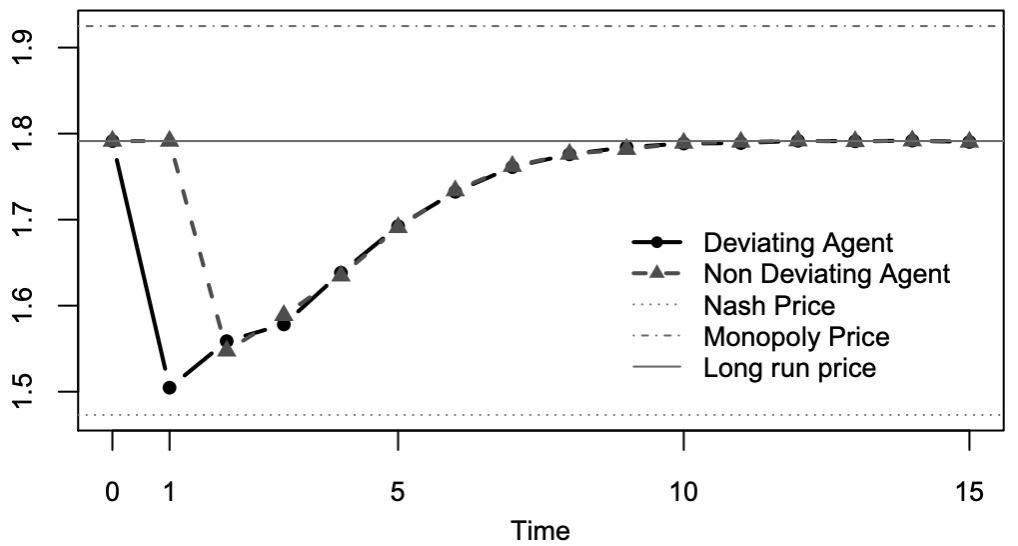
\includegraphics[width=1\linewidth]{image/calvano_impulse.png}
            \caption{Prices charged after an exogenous price cut by one agent in period $t = 1$.}
            \label{fig:calvano_impulse}
        \end{figure}

        Figure \ref{fig:calvano_impulse} shows one agent deviating at $t=1$.
        The results confirmed that when one agent deviated, the other agent responded by also reducing its price, effectively implementing punishment.
        Moreover, the deviating agent anticipated this punishment and began increasing its price in the next step after the forced reduction.
        This evidence supports the conclusion that agents learn collusive strategies.

    \subsection{Collusion by Other Algorithms}
        Whereas Calvano et al \cite{calvano2020a}. demonstrated the learning of collusive strategies in the repeated Bertrand model using Q-learning, Hettich et al. \cite{hettich2021} showed similar results using DQN.
        The time required for collusion to emerge was approximately 20,000 steps, which was significantly faster than that of Q-learning, which completed learning in an average of 850,000 steps.
        Furthermore, agents using DQN were confirmed to learn efficient reward--punishment schemes,
        demonstrating that DQN can learn collusive strategies similarly to Q-learning.

        The implementation of DQN enabled simulations with five or more agents.
        The results showed that $\Delta$ decreases as the number of agents increases, with $\Delta$ falling below 10\% with six or more agents.

        Hettich et al. examined the following methods as potential approaches to strengthening collusion among multiple agents:
        \begin{enumerate}
            \item Increasing the number of nodes and layers in the network.
            \item Extending the training period.
            \item Implementing double DQN.
            \item Modifying the state representation.
        \end{enumerate}

        The results indicated that methods 1, 2, and 3 did not significantly increase $\Delta$, whereas method 4 did.
        Hettich changed the state representation from \[\mathcal{P} \rightarrow  (\min{\mathcal{P}},mean{\mathcal{P}},\max{\mathcal{P}})\].
        Additionally, it was reported that DQN agents learn strong collusion even in markets where rule-based agents coexist.
\fi

% chapter 3
% ここにあった実験設定Settings of experimentはsection 5に移動しました

% chapter 4
\section{State Representation of Min and Second Min}
    % Methodologyとは日本語でいうところの「方法論」。提案手法ということでいいのか？ →修正しました。
    %First, we describe our proposed state representation, followed by a brief explanation of the process that led to this proposal.

    %\subsection{State Representation of Min and Second Min}
       We propose a state representation that increases $\Delta$ in wide markets.
        Hettich found that using the state representation
        $(\min{\mathcal{P}},mean{\mathcal{P}},\max{\mathcal{P}})$
        led to an increase in $\Delta$. 
        % (査読後)matcal{P}の説明を追加
        Here, $\mathcal{P}$ represents the set of prices $p_i$ offered by each firm $i$ in a market with $n$ firms, i.e., $\mathcal{P} = \{p_1, p_2, \ldots, p_n\}$.
        Hereafter, we refer to this state representation proposed by Hettich as MMM, taking the initials of three statistics (Min, Mean, and Max).
        %なぜか少し図の上下がずれます、、、 image/NN_MMMandMSM.pngを使えば横に揃えた表示はできますが、、、
        \begin{figure}[tb]
            \centering
            \begin{minipage}[b]{0.48\linewidth}
                \centering
                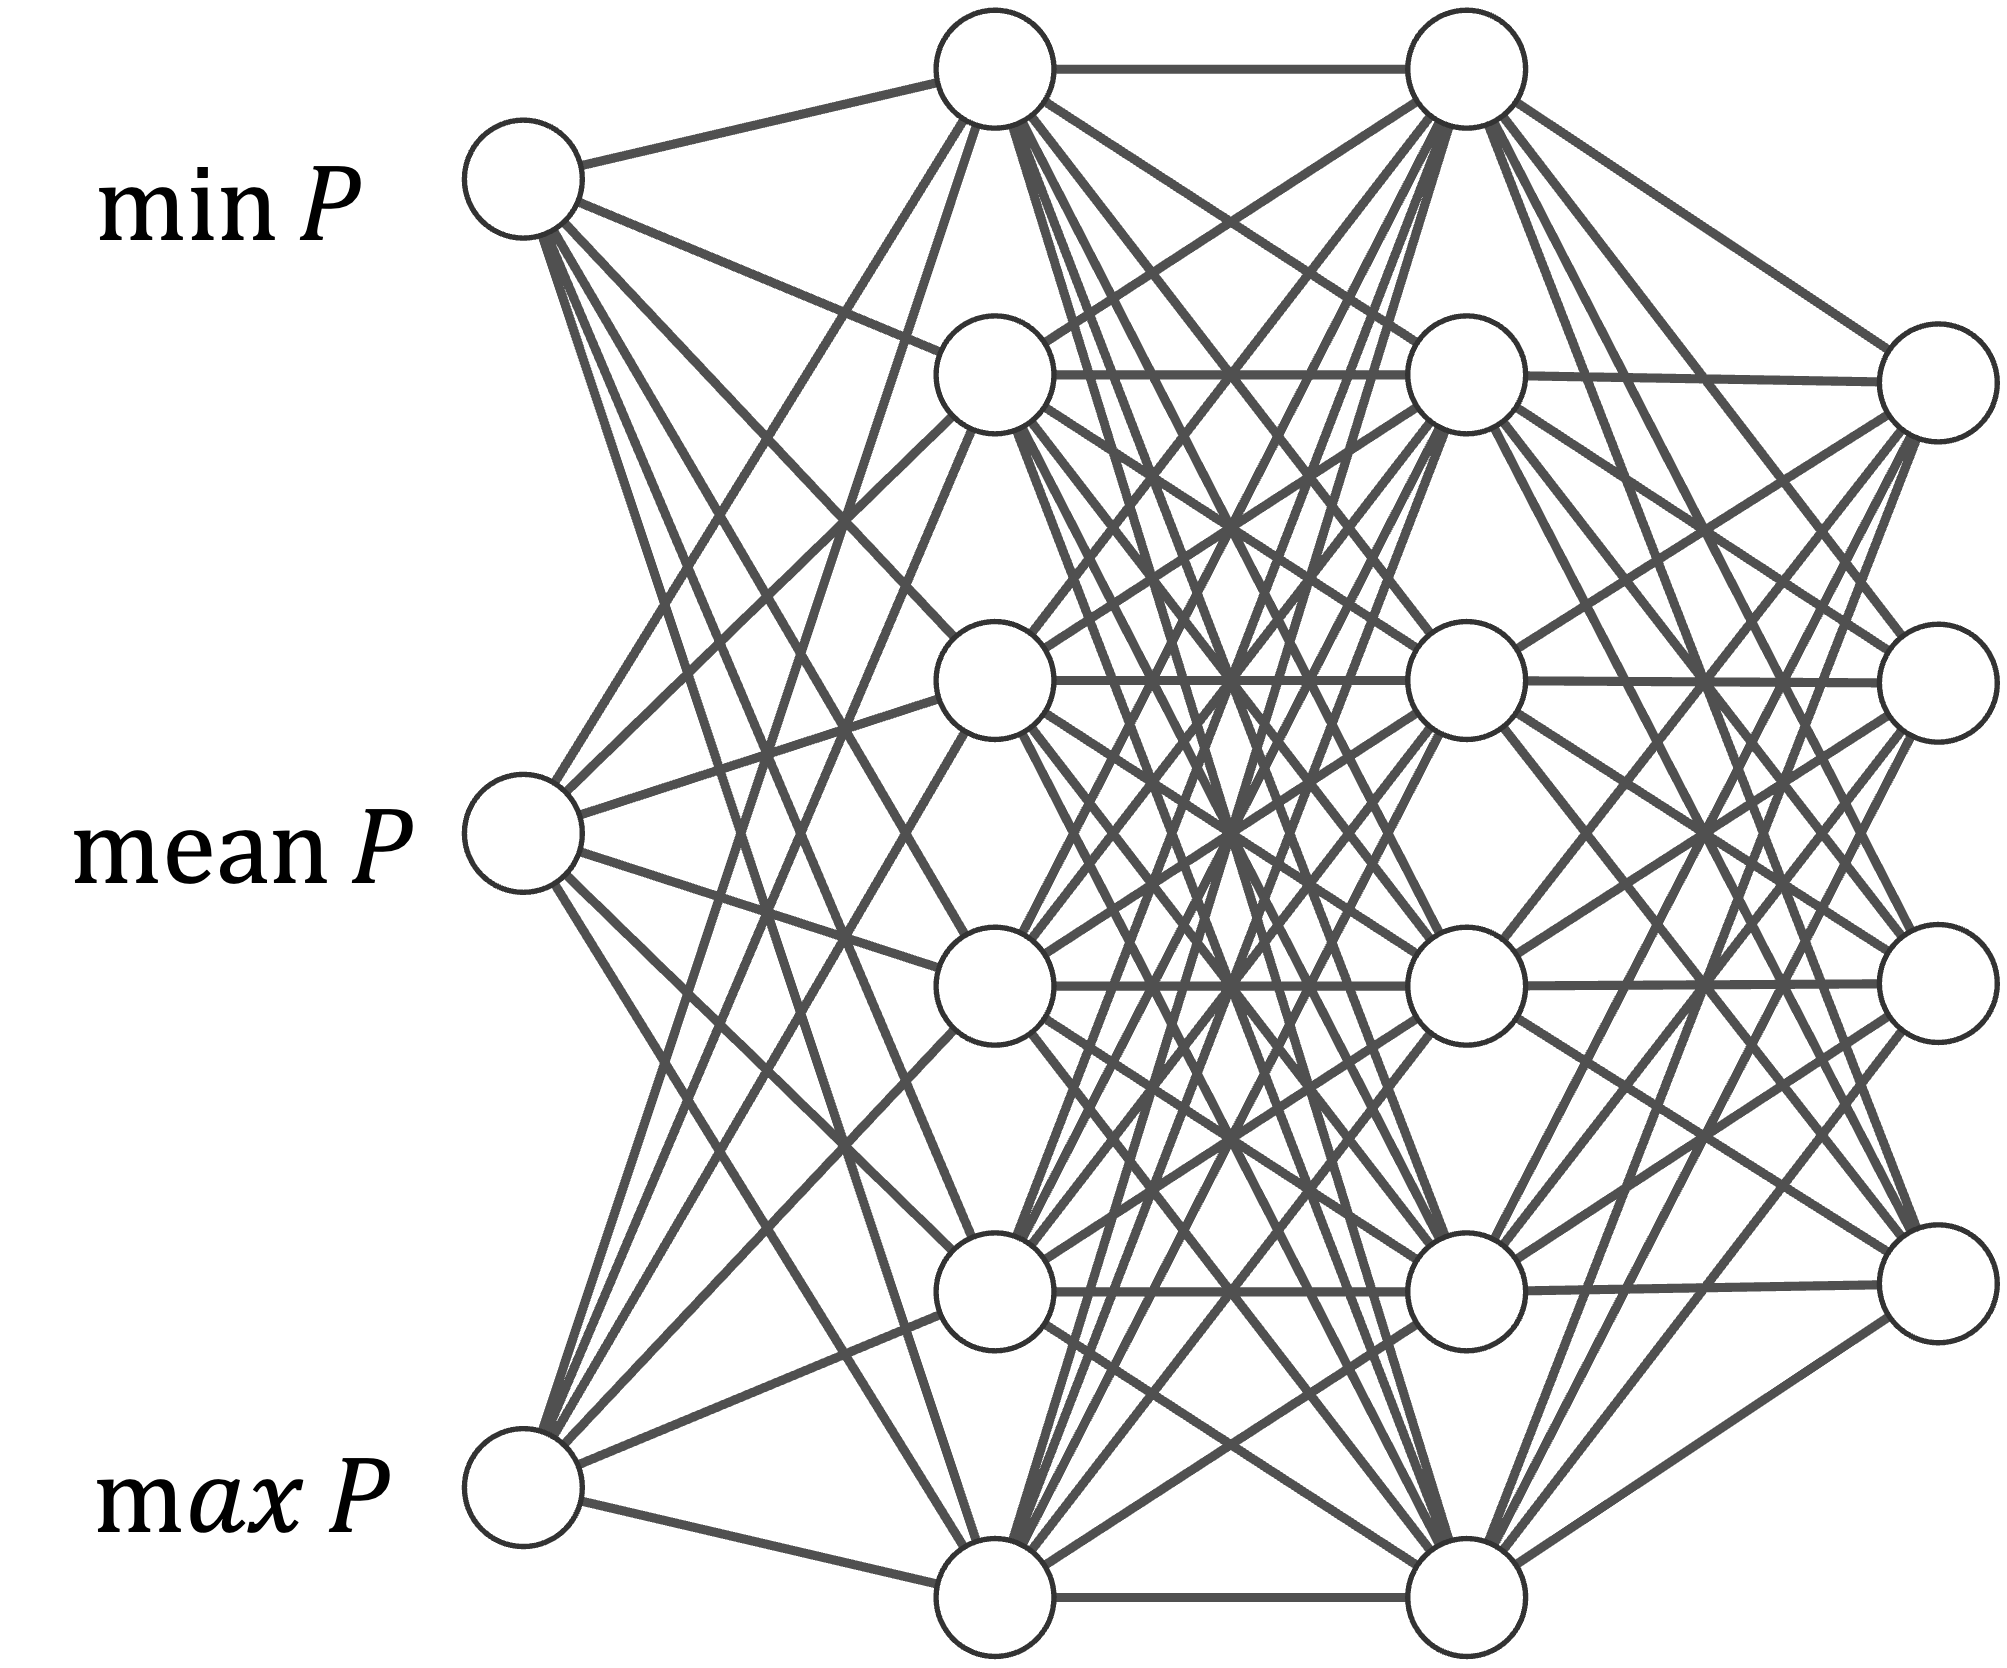
\includegraphics[width=\linewidth]{image/NN_MMM.png}
                \caption{Schematic diagram of a neural network using MMM state representation}
                \label{fig:MMM_NN}
            \end{minipage}%
            \hfill
            \begin{minipage}[b]{0.48\linewidth}
                \centering
                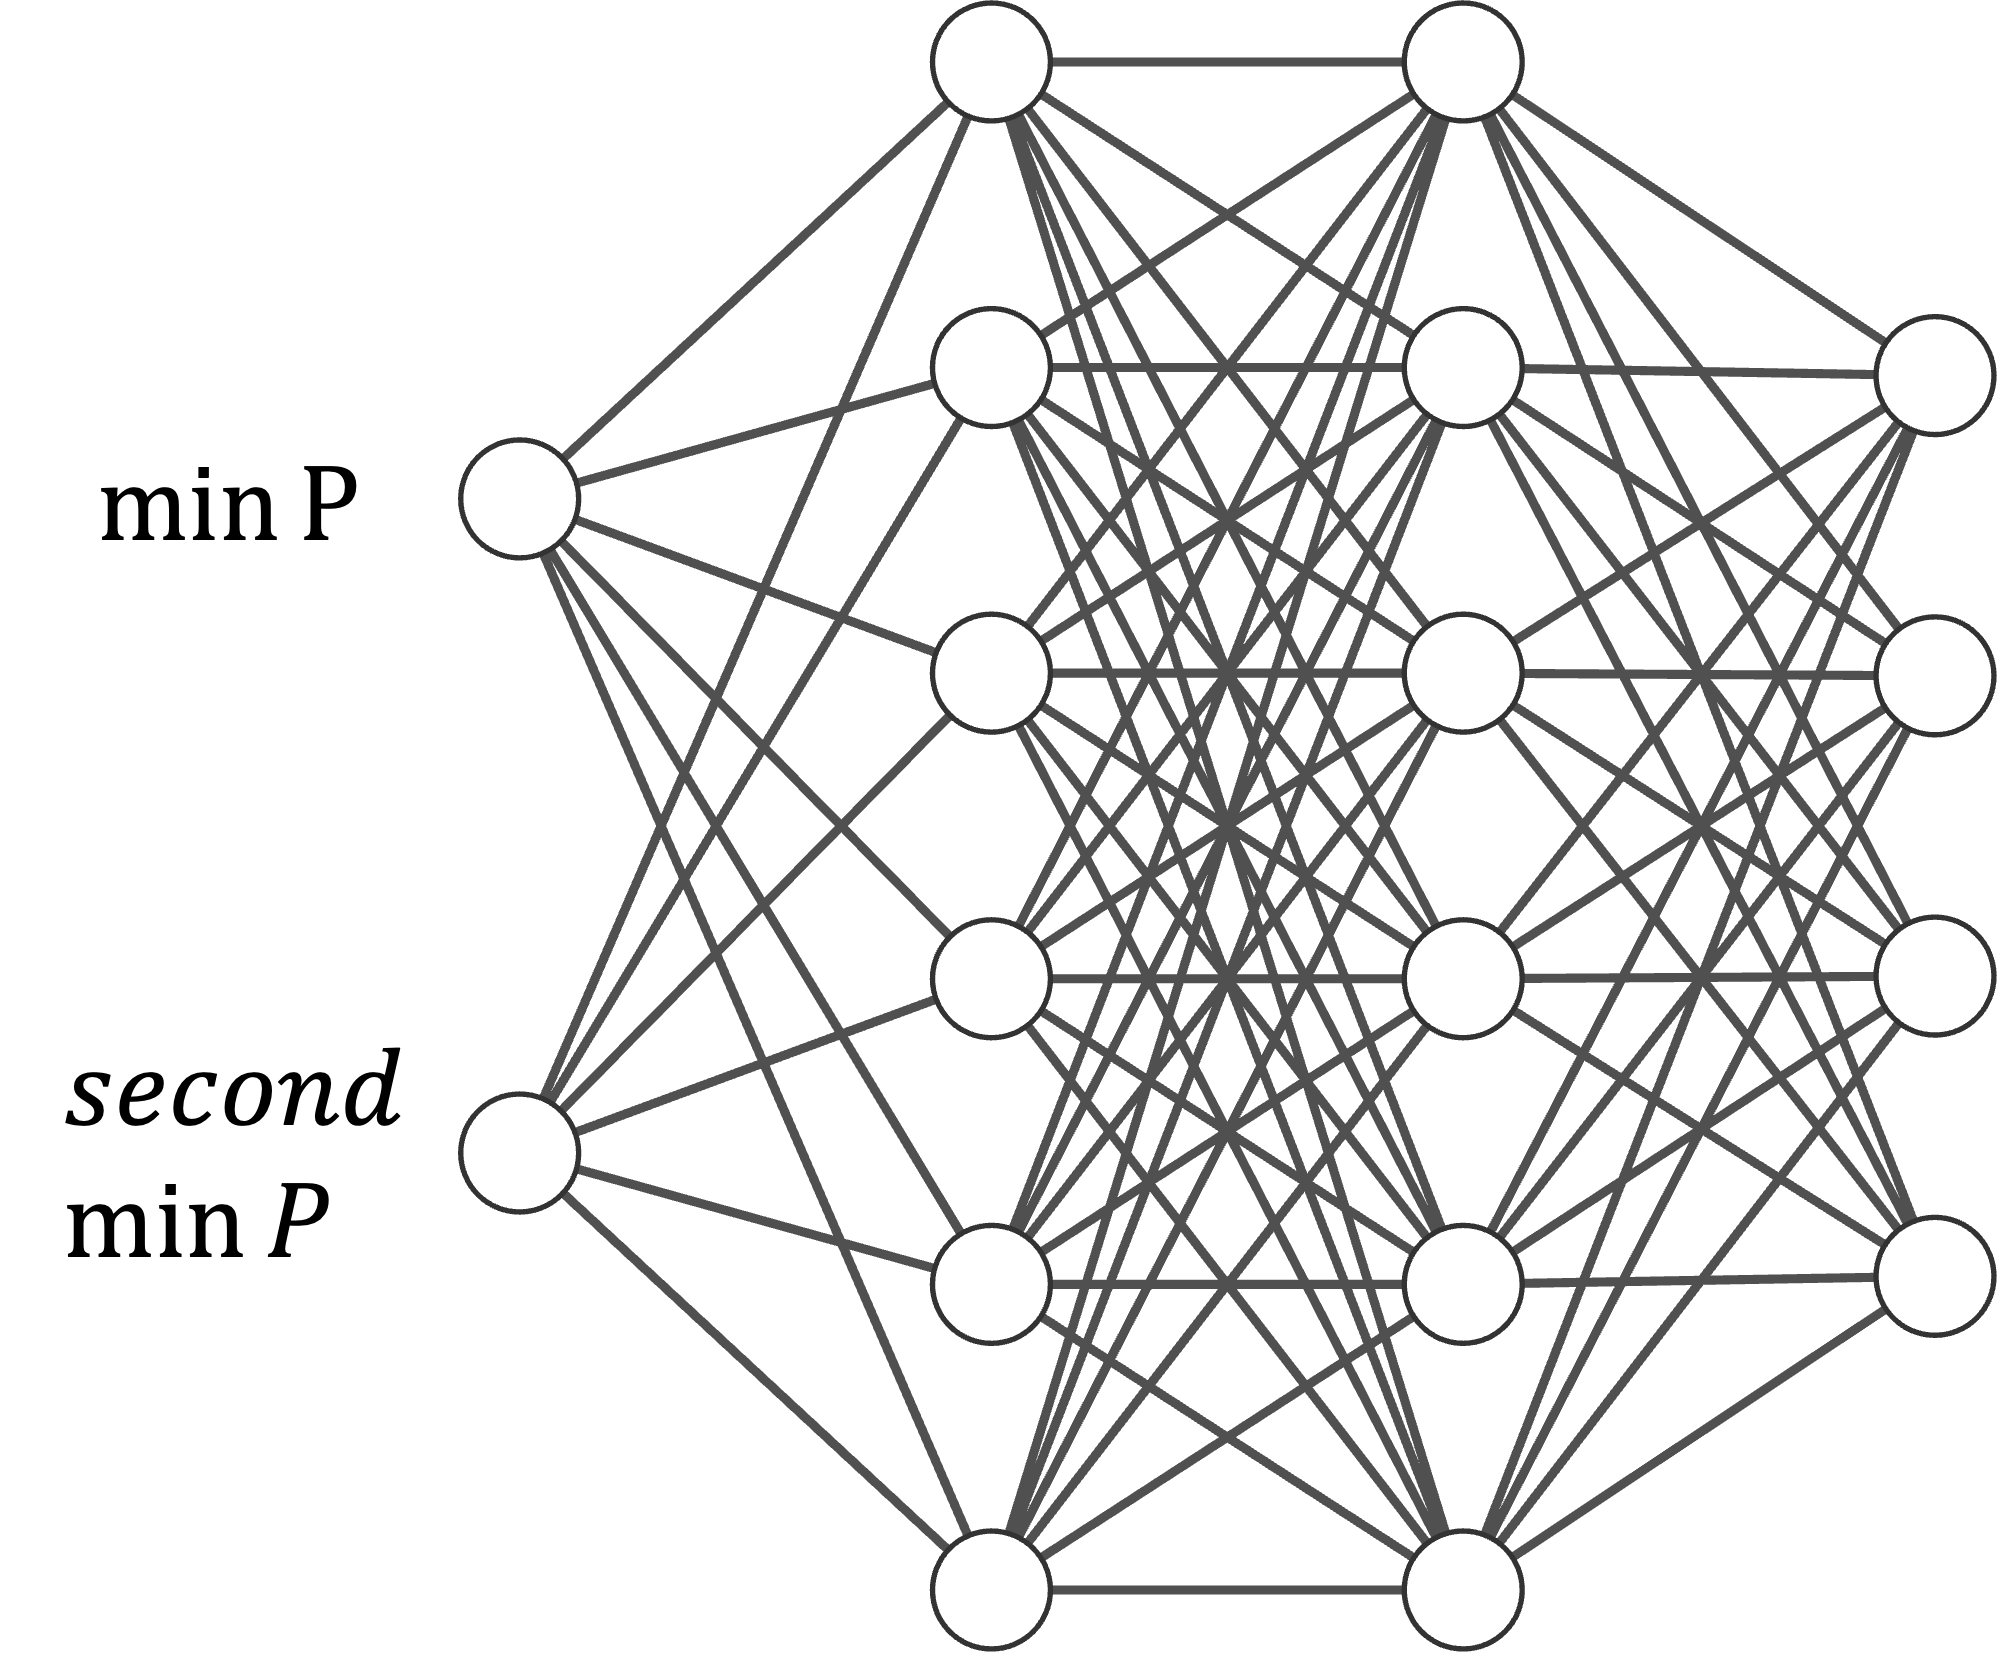
\includegraphics[width=\linewidth]{image/NN_MSM.png}
                \caption{Schematic diagram of a neural network using the proposed MSM state representation}
                \label{fig:MSM_NN}
            \end{minipage}
        \end{figure}

        We propose a state representation that includes the $k$ smallest values when the prices are sorted.
        For a set of prices \( \mathcal{P} \) with \( n \) elements, let \( \mathcal{P}^{\text{sorted}} \) denote the array of elements from set \( \mathcal{P} \) sorted in ascending order,
        and let \( \mathcal{P}^{\text{sorted}}_k \) denote the first \( k \) elements from this sorted array.
        For example, \( \mathcal{P}^{\text{sorted}}_1 = \min{\mathcal{P}} \).

        In the preliminary experiments, we mainly focus on the case where $k=2$ ($ \mathcal{P}_2^{\text{sorted}}$),
        which we specifically name MSM (state representation of Min and Second Min).
        When using this state representation, the neural network in Q-learning takes the form shown in Figure \ref{fig:MSM_NN},
        where the number of input nodes remains constant regardless of the number of agents.
        We propose using the lowest price and the second lowest price as the state representation.


\subsection{Preliminary Experiments}
    Before finding that \( \mathcal{P}^{\text{sorted}}_k \) leads to higher $\Delta$, we tested various state representations.
    Initially, we conducted simulations with different combinations of the three statistics (Min, Mean, and Max) used in Hettich's experiments and observed the resulting $\Delta$.
    Table \ref{tab:result_pre_experiment} shows the experimental results.
    The simulation involved three agents, with 32 simulations per state representation, and the other detailed experimental settings were identical to those described in Section \ref{sec:experiment}.
 
 
    \begin{table}[tb]
        \centering
        \caption{Statistics for each state representation}
        \label{tab:result_pre_experiment}
        \begin{tabular}{c|cc}
            \hline
            State Representation & Mean $\Delta$ & Standard Deviation of $\Delta$ \\
            \hline
            $(\max\mathcal{P})$ & 0.192872811 & 0.085955218 \\
            $(mean\mathcal{P})$ & 0.261742432 & 0.117688379 \\
            $(mean{\mathcal{P}},\max{\mathcal{P}})$ & 0.327645302 & 0.117169733 \\
            $(\min\mathcal{P})$ & 0.424324696 & 0.089198912 \\
            $(\min{\mathcal{P}},\max{\mathcal{P}})$ & 0.382954338 & 0.097241859 \\
            $(\min{\mathcal{P}},mean{\mathcal{P}})$ & 0.415223517 & 0.088598185 \\
            $(\min{\mathcal{P}},mean{\mathcal{P}},\max{\mathcal{P}})$ & 0.379652772 & 0.118152555 \\ \hline
        \end{tabular}
    \end{table}

    In Table \ref{tab:result_pre_experiment}, the inclusion of the minimum value significantly affects $\Delta$.
    Notably, state representations using only $\max{\mathcal{P}}$ or $mean{\mathcal{P}}$ show low $\Delta$ values, indicating insufficient learning of collusion.
    The highest $\Delta$ value was achieved with $(\min{\mathcal{P}})$, whereas state representations, including additional statistics, showed lower $\Delta$ values.
    Even Hettich’s MMM representation showed lower $\Delta$ values than state representations with a minimum value and one additional statistic.
    This means that including nonminimum statistics prevents the maintenance of higher $\Delta$.
    The mean value did not accurately consider the price changes of other agents as it did not directly reflect the actual prices set by agents.
    Given these results, we experimented with state representations, including the $k$ smallest values from the sorted prices.
    We conducted experiments with both three and nine firms. The nine-firm scenario was included to better observe the effects of increasing $k$, which might not be fully captured in the three-firm case.
    The results are shown in Table \ref{tab:result_pre_experiment2_9firm}.

%3社間の実験結果はスペースによっては削除かも→削除しました(喜多村)
    % \begin{table}[tb]
    %     \centering
    %     \caption{Mean and standard deviation of $\Delta$ for each state representation (\( \mathcal{P}^{\text{sorted}}_k \)) in a three-firm competition}
    %     \label{tab:result_pre_experiment2_3firm}
    %     \begin{tabular}{c|cc}
    %         \hline
    %         State Representation & Mean $\Delta$ & Standard Deviation of $\Delta$ \\
    %         \hline
    %         (\( \mathcal{P}^{\text{sorted}}_1 \)) & 0.3919 & 0.0985 \\
    %         (\( \mathcal{P}^{\text{sorted}}_2 \)) & 0.4686 & 0.0903 \\
    %         (\( \mathcal{P}^{\text{sorted}}_3 \)) & 0.4445 & 0.1046 \\
    %         \hline
    %     \end{tabular}
    % \end{table}

    \begin{table}[tb]
        \centering
        \caption{Mean and standard deviation of $\Delta$ for each state representation (\( \mathcal{P}^{\text{sorted}}_k \)) in a nine-firm competition}
        \label{tab:result_pre_experiment2_9firm}
        \begin{tabular}{c|cc}
            \hline
            State Representation & Mean $\Delta$ & Standard Deviation of $\Delta$ \\
            \hline
            (\( \mathcal{P}^{\text{sorted}}_1 \)) & 0.0597 & 0.0439 \\
            (\( \mathcal{P}^{\text{sorted}}_2 \)) & 0.0717 & 0.0454 \\
            (\( \mathcal{P}^{\text{sorted}}_3 \)) & 0.0714 & 0.0438 \\
            (\( \mathcal{P}^{\text{sorted}}_4 \)) & 0.0729 & 0.0454 \\
            (\( \mathcal{P}^{\text{sorted}}_5 \)) & 0.0687 & 0.0472 \\
            \hline
        \end{tabular}
    \end{table}

    In the three-firm case, $\Delta$ reached its maximum at $k = 2$. For the nine-firm scenario, $k = 4$ yielded the highest $\Delta$ value.
    However, in the nine-firm scenario, the variations in $\Delta$ values from $k = 2$ to $k = 5$ were minimal compared with the standard deviation,
    suggesting that $k = 4$ may not consistently yield the highest $\Delta$.
    These results indicate that including the second and subsequent smallest values in the state representation effectively promotes the learning of collusion strategies that achieve higher $\Delta$ values.
    The optimal state representation depends on the number of competing agents $n$.


% chapter 5
\section{Experiments}\label{sec:experiment}
    In this section, we first conduct experiments comparing the $\Delta$ values between MMM and MSM representations, followed by an analysis of the strategies acquired by agents under these different representations.
\subsection{Experimental Setting}
    We model the price competition between algorithms using a repeated Bertrand model based on Calvano et al. \cite{calvano2020a}.
    A multinomial logit model is used as the demand function.
    We fix the value of the outside good to $1$, following Hettich et al. \cite{hettich2021}, as follows:
    %The logit demand model with the outside good being $1$ is shown as follows:
    %\begin{equation}
    $d_{i,t} \left( p_{j \in n,t} \right) = e^{\frac{g_i - p_{i,t}}{\mu}}/(1 + \sum_{j=1}^{n} e^{\frac{g_j - p_{j,t}}{\mu}})$. 
    %\label{eq:fixed_logit_demand}
    %\end{equation}
    Sanchez-Cartas et al. \cite{Sanchez-Cartas2022} demonstrated that other demand models, such as linear demand models or Hotelling models, do not show significant increases in $\Delta$ as the logit demand model.
    %other demand functions such as linear demand models and Hotelling models.
    This makes it difficult to observe differences when the conditions are reformulated.
    Therefore, this study exclusively uses the logit demand model.
    When using DQN, discretizing price options are not strictly necessary, and continuous values can be simulated.
    Although environments using continuous values can better reflect reality, other existing studies using deep reinforcement learning algorithms have already demonstrated that similar collusive strategies can be learned in continuous action spaces as in discrete ones \cite{deng2024algorithmic,martello2022autonomous}.
    Therefore, to prioritize comparison with the state representation proposed by Hettich et al. \cite{hettich2021}, we use a discrete action space for the set of possible prices that agents can choose.
    We evaluate the results using the average profit gain $\Delta$ calculated from the mean of the last 100 periods of each simulation.

    Because of the significant variability in outcomes, all simulations are executed multiple times, and the average value is considered as $\Delta$ for that condition.
    Unless otherwise specified, each simulation is run 128 times.
    All DQN hyperparameters used are identical to those in Hettich et al. \cite{hettich2021}.


\subsection{Experimental Result}
\subsubsection{Three-Firm Condition}\label{sec:experiment_3firms}
%    This section shows that using our proposed state representation leads to increased collusion.
    We conducted simulations of our proposed MSM and MMM by Hettich et al. with three agents in an identical environment. 
%    \begin{enumerate}
%        \item Simulation using our proposed state representation (MSM).
%        \item Simulation using Hettich et al.'s state representation (MMM) \cite{hettich2021}.
%    \end{enumerate}
    During the simulations, we showed the average profit $\Delta$ for each agent.
    To make the differences more straightforward, we extended the simulation period to 300,000 periods.
    The evolution of $\Delta$ of every period is shown in Figure \ref{fig:result_3firm}.

    % hがその場所、　tが一番上、cが一番下
    % (査読後)スペースが足りないのでやむなく図のサイズを落としました
    \begin{figure}[tb]
        \centering
        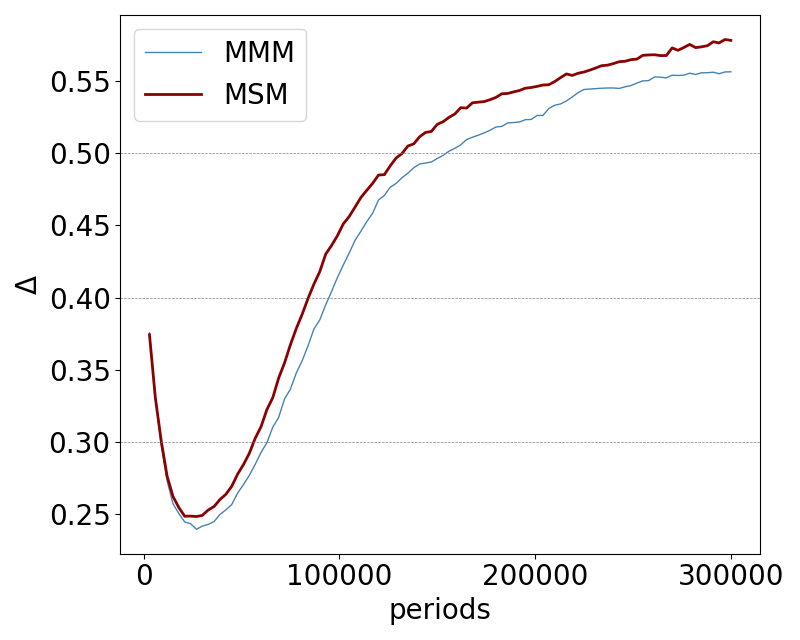
\includegraphics[width=0.5\linewidth]{image/3fi_300kiloperiods3.png}
        \caption{$\Delta$ with every period in three-firm experiments}
        \label{fig:result_3firm}
    \end{figure}

    \begin{table}[tb]
        \centering
        \caption{Statistical values from three-firm experiments}
        \label{tab:statistics_3firm}
        \begin{tabular}{clcc}
            \hline
            Statistic & MMM & MSM \\
            \hline
            Mean & 0.556168503 & 0.577526397 \\
            Standard deviation & 0.071096721 & 0.057385524 \\
            Minimum & 0.358977343 & 0.367677329 \\
            Maximum & 0.782678685 & 0.774478049 \\
            \hline
        \end{tabular}
    \end{table}

    % この辺の話は書かないで「検定を行った結果、優位な差が確認できた」の一文で済ませてもいいような気がしています。が一応残しました
    Table \ref{tab:statistics_3firm} shows the statistical values obtained by averaging the last 100 periods of each of the 128 simulations and agents.
    To verify whether there is a significant difference in the average profit $\Delta$ between the MMM and MSM conditions, we conducted Welch’s $t$-test, which yielded the following results: $t$-value was \($-$2.645\) and $p$-value was \(0.0087\). 
    %
    As the $p$-value was below the 1\% significance level (\(\alpha = 0.01\)), the difference in the means between the MMM and MSM was statistically significant.
    Therefore, the adoption of MSM led to a statistically significant increase in $\Delta$ compared with MMM.    
    The rise in $\Delta$ could be attributed to the enhanced detection of deviations from the collusion by other firms.
   %
    Figure \ref{fig:result_3firm} shows that the $\Delta$ values were nearly identical until around 20,000 timesteps when the collusion began.
    This means that MSM state representation performs similarly to MMM during competitive learning, with differences manifesting only during the learning of collusive strategies.

\subsubsection{Price Reaction after the Defection of One Agent}
    The increase in $\Delta$ is insufficient to prove that agents have truly learned collusive strategies.
    Two possible explanations exist for the convergence to prices higher than competitive levels:
    \begin{itemize}
        \item Agents failed to effectively learn competitive strategies.
        \item Agents learned effective reward--punishment schemes, resulting in collusion.
    \end{itemize}
    % 本来reward-punishment schemeとしたいが、それをやると一行の幅を超えると警告が出るので仕方がなく reward と punishment の間に空白を入れてしまっている
    Hettich et al. demonstrated that DQN can learn reward--punishment schemes \cite{hettich2021}.
    However, it remains unclear whether agents can learn effective reward--punishment schemes when the state representation is reformulated.

    We demonstrate that agents learn reward--punishment schemes even in environments implementing MSM by Calvano et al. \cite{calvano2020a}.
    The experimental requirements are as follows:
    \begin{itemize}
        \item To maintain consistency with Calvano et al.'s conditions, we use two agents.
        \item Agents are trained in advance for 100,000 periods, repeated 64 times.
        \item After training, the strategies are fixed for a 10-period test phase.
        \item At period 0, one agent’s price is forcibly reduced to the Nash equilibrium price.
        \item We measure the average price responses across 128 trained agents.
    \end{itemize}
    Unlike other experiments evaluated using $\Delta$, this analysis directly examines the prices set by agents.

    % (査読後)スペースが足りないのでやむなく図のサイズを落としました
    \begin{figure}[tb]
        \centering
        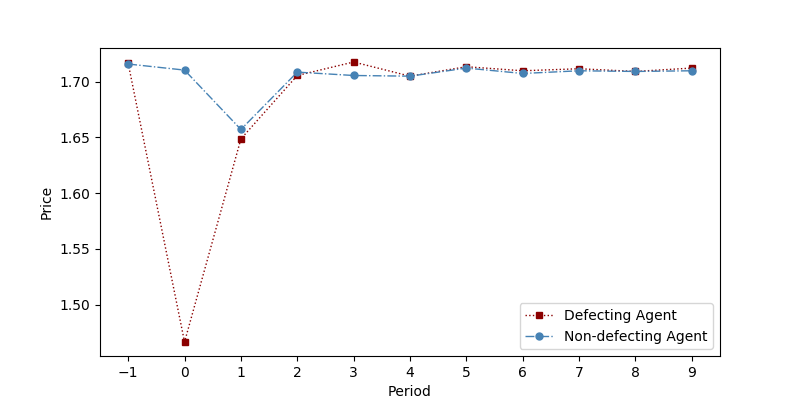
\includegraphics[width=0.8\linewidth]{image/minsec2agentdefectzoom2.png}
        \caption{Price response after agent deviation using MSM representation}
        \label{fig:rewardpunishment_zoom}
    \end{figure}

    Figure \ref{fig:rewardpunishment_zoom} shows the price responses obtained from the simulation experiments.
    The results shown in Figure \ref{fig:rewardpunishment_zoom} are similar reactions when using Q-learning.
    Specifically, after an agent deviates at $t=0$, the nondeviating agent responds by lowering its price at $t=1$.
    The deviating agent, anticipating this punishment, begins raising its price at $t=1$.
    Figure \ref{fig:rewardpunishment_zoom} shows that the convergence level after a deviation is slightly lower than the predeviation level.
    This phenomenon is consistent with Hettich’s observations when using the original state representation ($\mathcal{P}$).
    Therefore, we can conclude that agents using MSM representation successfully learn reward--punishment schemes to maintain collusion.
    % 卒論では"3社での実験"を複数やりましたが、この論文の主な主張を助けるための実験結果への影響は軽微だと思うのでここではこの一文↓で終わらせてしまおうと思います
    We also conducted experiments with three agents and similarly confirmed that reward-punishment learning was achieved.

    We demonstrate the learned strategies in the two-agent case.
    Figures \ref{fig:actionmap_normal} and \ref{fig:actionmap_msm} show the optimal actions $a = \arg\max_a Q(s, a, \theta)$ for each state in a $15 \times 15$ grid for agents trained using ($\mathcal{P}$) and MSM representations, respectively.

    \begin{figure}[tb]
        \centering
        \begin{minipage}{0.45\linewidth}
            \centering
            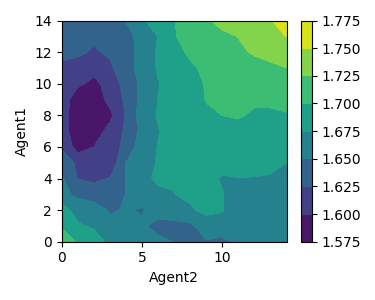
\includegraphics[width=1\linewidth]{image/2fi_actionmap_normal_mini.png}
            \caption{Optimal actions of Agent 1 using ($\mathcal{P}$) representation}
            \label{fig:actionmap_normal}
        \end{minipage}
        \hfill
        \begin{minipage}{0.45\linewidth}
            \centering
            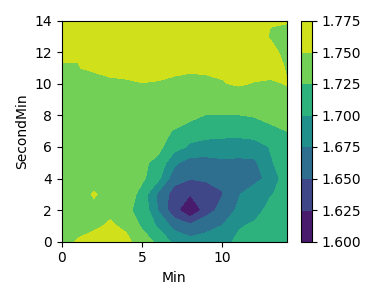
\includegraphics[width=1\linewidth]{image/2fi_actionmap_minsec_mini.png}
            \caption{Optimal actions of Agent 1 using MSM representation}
            \label{fig:actionmap_msm}
        \end{minipage}
    \end{figure}

    The results in Figure \ref{fig:actionmap_normal} are consistent with those demonstrated by Hettich et al. \cite{hettich2021}.
    In Figure \ref{fig:actionmap_msm}, the regions where $min>second~min$ remain unlearned, which is expected given this logical impossibility.
    This confirms that MSM representation is effectively incorporated into the learning process.
    It reveals that agents learn to set higher prices when both the minimum and second minimum values are low.
    This is also seen in Figure \ref{fig:actionmap_normal}, which indicates that agents encourage the resumption of collusion by setting high prices when both agents have previously offered low prices.
    The regions showing optimal actions with lower prices represent punishments triggered when each agent deviates with a low price.

    % ↓これは"3社での実験" 

    % To analyze the differences resulting from state representation changes, we conduct experiments with a one-period price reduction above the Nash equilibrium price.
    % The experimental requirements are as follows:
    % \begin{itemize}
    %     \item Three agents are used to clearly observe differences between MMM and MSM
    %     \item Agents undergo preliminary training for 100,000 periods, repeated 64 times
    %     \item After training, strategies are fixed for a 30-period test phase
    %     \item At period 15, one agent's price is forcibly reduced to a predetermined level
    %     \item Price responses are averaged over 512 total trials (8 trials for each of the 64 trained agents)
    % \end{itemize}

    % \begin{figure}[htbp]
    %     \centering
    %               \begin{minipage}{\linewidth}
    %                 \centering
    %                 \includegraphics[width=0.9\linewidth]{image/impulse/minsec3fiexp.png}
    %               \end{minipage}

    %               \begin{minipage}{\linewidth}
    %                 \centering
    %                 \includegraphics[width=0.9\linewidth]{image/impulse/refo3fiexp.png}
    %               \end{minipage}

    %               \begin{minipage}{\linewidth}
    %                 \centering
    %                 \includegraphics[width=0.9\linewidth]{image/impulse/normal3fiexp.png}
    %               \end{minipage}
    %     \caption{Experimental results under Condition 2 (from top: MSM, MMM, ($\mathcal{P}$))}
    %     \label{fig:condition2}
    % \end{figure}

    % Figure \ref{fig:condition2} demonstrates that when prices are reduced to a level above the Nash price, both MSM and MMM agents exhibit price reductions by non-deviating agents.
    % This behavior indicates successful learning of reward-punishment schemes.
    % Notably, MSM agents implement more substantial price reductions compared to MMM agents.
    % This difference in punishment severity likely contributes to the enhanced collusive behavior observed in the MSM representation.

\subsubsection{Multifirm Condition}

    We conducted experiments with four to ten agents to demonstrate that MSM generates stronger collusion even with an increased number of firms.
    For each number of agents, 128 simulations were performed. The learning algorithm and other parameters used were the same as those with three-firm conditions.

    % (査読後)スペースが足りないのでやむなく図のサイズを落としました
    \begin{figure}[tb]
        \centering
        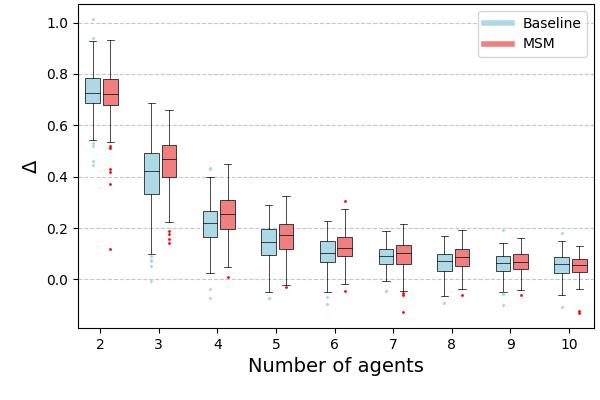
\includegraphics[width=0.6\linewidth]{image/resultmanyfirm2.png}
        \caption{Average profit $\Delta$ with four or more firms}
        \label{fig:result_manyfirm}
    \end{figure}

    Figure \ref{fig:result_manyfirm} shows that MSM achieves a higher average profit $\Delta$ than MMM, even with four or more firms.
    However, the difference between MSM and MMM tends to decrease as more agents are added, becoming negligible with ten firms.
    As the number of agents increases, the average profit $\Delta$ decreases. This means that the reduction in difference might be proportional to this scale-down.
    Table \ref{tab:change_rate} shows the rate of change in the collusion levels of MSM compared with the baseline.
    
    \begin{table}[tb]
    \small
    \centering
    \caption{Rate of change in collusion levels between MMM and MSM for different numbers of firms}
    \label{tab:change_rate}
    \begin{tabular}{|p{3cm}|*{9}{c|}}
        \hline
        Number of Firms & 2 & 3 & 4 & 5 & 6 & 7 & 8 & 9 & 10 \\
        \hline
        MMM & 0.73 & 0.41 & 0.21 & 0.14 & 0.10 & 0.08 & 0.07 & 0.06 & 0.05 \\
        MSM & 0.72 & 0.45 & 0.26 & 0.17 & 0.12 & 0.10 & 0.08 & 0.07 & 0.06 \\
        Change rate (\%) & $-0.99$ & 10.02 & 25.56 & 23.17 & 22.09 & 20.38 & 17.79 & 15.16 & 10.17 \\
        \hline
    \end{tabular}
    \end{table}
        
    MSM showed the highest increase rate with four firms.
    The higher increase rate in the four-firm case compared with the three-firm case could be attributed to the same reason for the low increase rate in the two-firm case: the similarity between the statistical values taken by MSM and MMM.
    In the three-firm case, the mean value used in MMM, the average of the minimum and maximum values, tended to be close to the second minimum value used in MSM.
    However, with four or more firms, the difference between the mean value and the second minimum value became more pronounced, leading to a higher increase in collusion levels.
    Beyond the four firms, the enhancement in collusion levels gradually diminished, even when considering the rate of change.

    \begin{table}[tb]
        \centering
        \caption{Average profit $\Delta$ with varying $k$ in \( \mathcal{P}^{\text{sorted}}_k \) for different numbers of agents}
        \label{tab:experiment_variable_k}
        \begin{tabular}{|c|c|c|c|c|c|c|c|c|c|}
            \hline
            %(査読後) 列がエージェント数でもあるとわかりやすいように表中にnb.agents(number of agents)を追加　(状態表現が含む値の数でもあるので)
            $k$ \textbackslash\ nb.agent & 3 & 4 & 5 & 6 & 7 & 8 & 9 & 10 \\
            \hline
            2 & 0.4535 & 0.2628 & 0.1700 & 0.1241 & 0.0986 & 0.0828 & 0.0675 & 0.0580 \\
            3 & 0.4478 & 0.2501 & 0.1660 & 0.1256 & 0.0990 & 0.0826 & 0.0729 & 0.0632 \\
            4 &  & 0.2147 & 0.1459 & 0.1125 & 0.0947 & 0.0793 & 0.0704 & 0.0605 \\
            5 &  &  & 0.1405 & 0.1018 & 0.0870 & 0.0773 & 0.0661 & 0.0591 \\
            \hline
        \end{tabular}
    \end{table}
    
   To investigate further, unlike previous experiments, this study conducted tests with varying values of $k$ in \( \mathcal{P}^{\text{sorted}}_k \). 
    Table \ref{tab:experiment_variable_k} reveals that when the number of firms is $5$ or fewer, $k=2$ (MSM representation) produces the highest $\Delta$.
    When the number of firms exceeds 5, the state representation with $k=3$ yields higher $\Delta$.
    % interestingは主観的な表現だから論文には適さない...?  => importantでいいとおもいます。
    This finding of the optimal state representations with the number of firms in the market is particularly important.
   Considering the experimental results, the optimal representation depends on the number of competing firms.

% chapter 6
\section{Conclusion}
We proposed that the reformulation of state representation affects the learning of collusion strategies.
Our results showed that agents achieve higher profits when they adopt a state representation focusing on MSM rather than the conventional combination of minimum, mean, and MMM.
We confirmed that the learned strategies include reward--punishment schemes that promote collusion.
Furthermore, MSM representation increased profits compared with MMM, even in markets with more than two agents.
We demonstrated that the optimal state representation varies according to the number of participating agents in the market.

However, because of computational time constraints, our experiments were limited to markets with up to ten agents. Thus, future work must investigate the relationship between the number of agents and the optimal value of $k$ in larger markets.
Moreover, although our experiments utilized the DQN approach, numerous other reinforcement learning algorithms exist.
Policy-based learning algorithms have been increasingly adopted in recent studies \cite{deng2024algorithmic,martello2022autonomous}.
Further research is needed to verify whether our proposed state representation enables the learning of strategies that increase profits when using algorithms other than DQN.

Profits increased in multiagent price competition merely by modifying the state representation without changing the learning algorithm, raising concerns about the growing risk of algorithmic collusion.
Given the finding that focusing on lower prices and closely related prices promotes collusion, regulatory approaches that restrict updates or access to lower price information may prove effective in mitigating these risks.


% creditってここに書くので合っていますかね...?→査読通過後で大丈夫です
\begin{credits}
\subsubsection{\ackname}
This work was supported by JSPS KAKENHI Grant Numbers 24K22333, 22H03641, 21K19818, and JST FOREST (Fusion Oriented REsearch for disruptive Science and Technology) Grant Number JPMJFR216S.
\end{credits}


% ---- Bibliography ----

% BibTeX users should specify bibliography style 'splncs04'.
% References will then be sorted and formatted in the correct style.

\bibliographystyle{splncs04}
\bibliography{main}

\end{document}
